\documentclass[12pt]{article}			% For LaTeX 2e
						% other documentclass options:
						% draft, fleqn, openbib, 12pt

\usepackage{graphicx}	 			% insert PostScript figures
\usepackage{caption}
\usepackage{subcaption}
\usepackage{wrapfig}
\usepackage{amsmath}
%% \usepackage{setspace}   % controllabel line spacing
%% If an increased spacing different from one-and-a-half or double spacing is
%% required then the spacing environment can be used.  The spacing environment 
%% takes one argument which is the baselinestretch to use,
%%         e.g., \begin{spacing}{2.5}  ...  \end{spacing}


% the following produces 1 inch margins all around with no header or footer
\topmargin	=10.mm		% beyond 25.mm
\oddsidemargin	=0.mm		% beyond 25.mm
\evensidemargin	=0.mm		% beyond 25.mm
\headheight	=0.mm
\headsep	=0.mm
\textheight	=220.mm
\textwidth	=165.mm
					% SOME USEFUL OPTIONS:
% \pagestyle{empty}			% no page numbers
 \parindent  15.mm			% indent paragraph by this much
 \parskip     2.mm			% space between paragraphs
% \mathindent 20.mm			% indent math equations by this much

\newcommand{\MyTabs}{ \hspace*{25.mm} \= \hspace*{25.mm} \= \hspace*{25.mm} \= \hspace*{25.mm} \= \hspace*{25.mm} \= \hspace*{25.mm} \kill }

\graphicspath{{../Figures/}{../data/:}}  % post-script figures here or in /.

					% Helps LaTeX put figures where YOU want
 \renewcommand{\topfraction}{0.9}	% 90% of page top can be a float
 \renewcommand{\bottomfraction}{0.9}	% 90% of page bottom can be a float
 \renewcommand{\textfraction}{0.1}	% only 10% of page must to be text

\linespread{1.2}
\alph{footnote}				% make title footnotes alpha-numeric

\begin{document}			% REQUIRED

\begin{center}
	{\LARGE \bf Results}
\end{center}

\section{Hard Biometrics}
\begin{figure}[h]
	\centering
	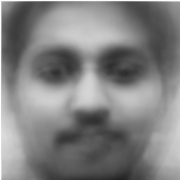
\includegraphics[scale=0.8]{img/avg.jpeg}
	\caption{ \small The average of all trained faces } 
	\label{fig:hb1}
\end{figure}

\begin{figure}[b]
	\centering
	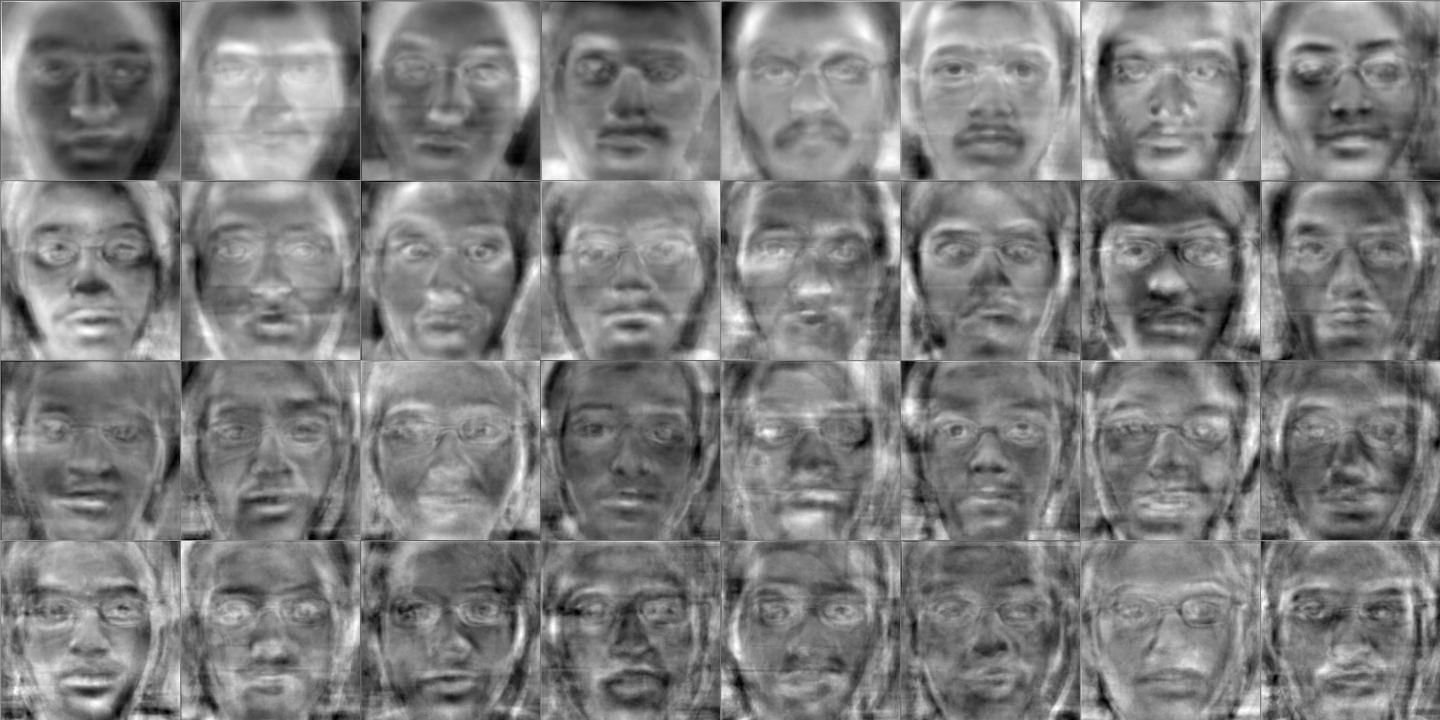
\includegraphics[scale=0.3]{img/eigen.png}
	\caption{ \small $N$ eigenfaces are created to represent the deviation, where $N$ is the number of training images } 
	\label{fig:hb2}
\end{figure}

\begin{figure}[h]
	\centering
	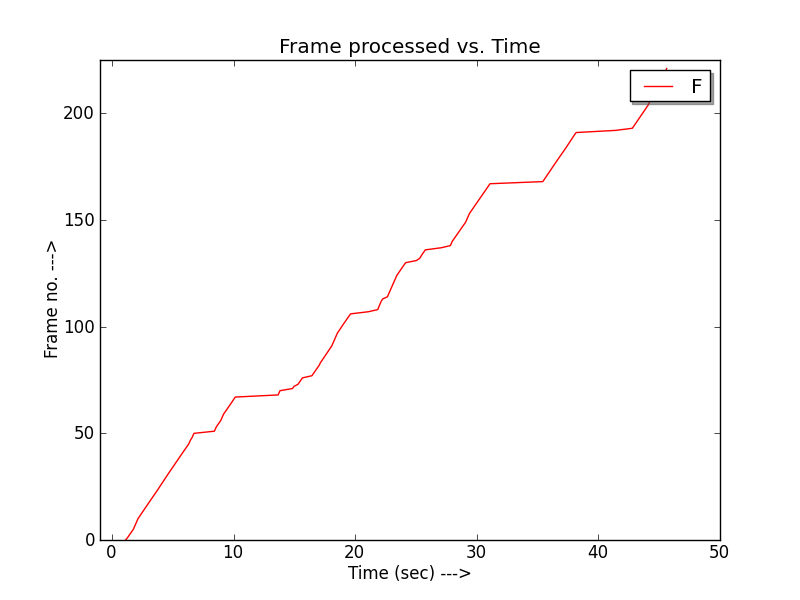
\includegraphics[scale=0.5]{img/t_fno.png}
	\caption{ \small Number of frames processed over time}
	\label{fig:hb3}
\end{figure}

\begin{figure}[h]
	\centering
	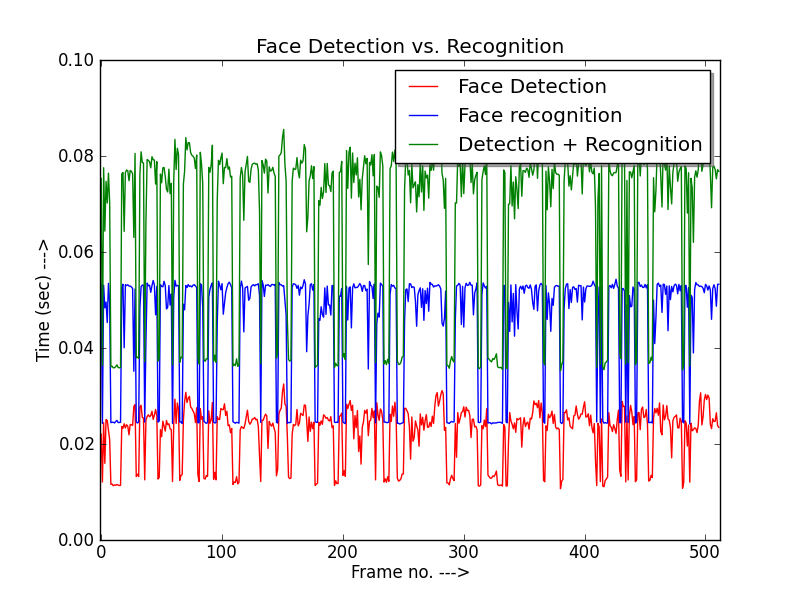
\includegraphics[scale=0.5]{img/fd_fr_fdfr.png}
	\caption{ \small Comparison of time taken to process facial features }
	\label{fig:hb4}
\end{figure}

\begin{figure}[t]
	\centering
	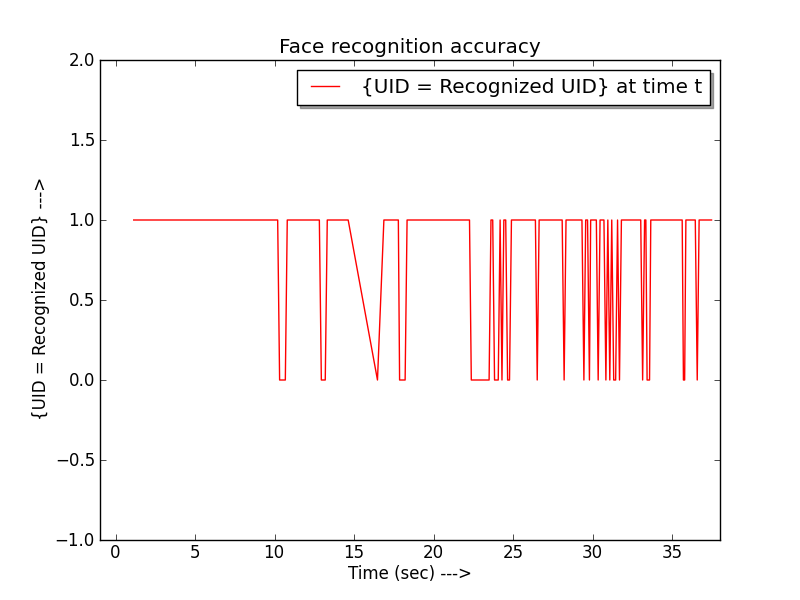
\includegraphics[scale=0.5]{img/face_rec_accuracy.png}
	\caption{ \small Authentication cannot be solely determined by output from Face recognition due to noise. }
	\label{fig:hb5}
\end{figure}

\end{document}
